\chapter{Introduction to Binary Classification}

The problem of data classification is very important in the modern world. The classification aims to find a relation between a set of objects and target variables based on some objects' properties. The properties of the objects are usually called features, and the target variables are usually called labels. Many real-world problems can be formulated as classification tasks:
\begin{itemize}
  \item \textbf{Medical Diagnosis:} In medicine, the classification is often used to improve disease diagnosis. In such a case, the features are medical records such as the patient's blood tests, temperature, or roentgen images. The target variable is if the patient has some disease. For example, classification can be used to process mammogram images and detect cancer~\cite{viale2012current, levy2016breast}.
  \item \textbf{Internet Security:} These days, the internet is a crucial part of our lives. With the increasing usage of the internet, the number of attacks increases as well. An essential part of the defense is intrusion detection systems~\cite{grill2016learning, scarfone2007guide} that search for malicious activities (network attacks) in network traffic. Classification can be used to improve such systems as shown in~\cite{giacinto2002intrusion, shanbhag2009accurate}.
  \item \textbf{Marketing:} In marketing, the task can be to classify customers based on their buying interests. Such information can be used to build a personalized recommendation system for customers and therefore increase income~\cite{kaefer2005neural, zhang2007building}.
\end{itemize}
Besides these three examples, applications of classification can be found in almost every academic or even industrial field. Furthermore, a vast number of algorithms try to solve classifications problems. Typically these algorithms consist of three phases:
\begin{itemize}
  \item \textbf{Training:} The classification problems usually fall into the category of supervised learning. It means that we assume the prior knowledge of the target classes in the training phase. The training data typically consists of pairs (sample, label) and can be described as follows
  \begin{equation*}\label{eq: training set}
    \mathcal{D}_{\mathrm{train}} = \Brac[c]{(\bm{x}_i, y_i)}_{i=1}^{n},
  \end{equation*}
  where the sample~$\bm{x}_i \in \R^d$ is a~$d$-dimensional vector of features that describes the object of interes and the label~$y_i \in \{1, 2, \ldots, k\}$ represents target class. Moreover~$n \in \N$ is a number of training samples and~$k \in \N$ is a number of target classes. In this phase, the algorithm uses the training data to learn a model, i.e., set model parameters according to some predefined criterion, to describe the training data as best as possible.
  \item \textbf{Validation:} All algorithms usually have some hyperparameters that can be changed to improve the resulting model. The validation phase is used to select the best hyperparameter settings that lead to the most performant and robust model.
  \item \textbf{Testing:} In the testing phase, the model is used to assign labels~$\hat{y}_i \in \{1, 2, \ldots, k\}$ to the data from the testing set, which is not known during the training phase.
\end{itemize}
The previous definition of the training set is general for any classification problem with multiple classes. However, we focus on the special subclass of classification problems called binary classification in this work. The binary classification is a special case of classification in which the number of classes is~$k=2.$ These two classes are usually referred to as negative and positive classes. Moreover, the positive class is usually the one we are more interested. Returning to example with cancer, the positive class would represent that the patient has cancer while the negative that the patient is healthy.

\begin{notation}[Dataset]\label{not: dataset}
  In this work, we use label~$0$ to encode the negative class and label~$1$ to encode the positive class. Moreover, by a dataset of size~$n \in \N$ we mean a set of pairs in the following form
  \begin{equation*}
    \mathcal{D} = \Brac[c]{(\bm{x}_i, y_i)}_{i=1}^{n},
  \end{equation*}
  where~$\bm{x}_i \in \R^d$ represents samples,~$d \in \N$ its dimension and~$y_i \in \{0, 1\}$ corresponding labels. To simplify future notation, we denote a set of all indices of dataset~$\mathcal{D}$ as~$\I = \Ineg \cup \Ipos,$ where
  \begin{equation*}
    \begin{aligned}
      \Ineg & = \Set{i}{i \in \{1, 2, \ldots, n\} \; \land \; y_i = 0}, \\
      \Ipos & = \Set{i}{i \in \{1, 2, \ldots, n\} \; \land \; y_i = 1}.
    \end{aligned}
  \end{equation*}
  We also denote the number of negative samples in~$\mathcal{D}$ as~$\nneg = \Brac[v]{\Ineg}$ and the number of positive samples in~$\mathcal{D}$ as~$\npos = \Brac[v]{\Ipos},$ i.e. total number of samples is~$n = \nneg + \npos.$ 
\end{notation}

The goal of any classification problem is to classify given samples with the highest possible accuracy or, in other words, with the lowest possible error. In the case of binary classification, there are two types of error: positive sample is classified as negative and vice versa. Formally, using the Notation~\ref{not: dataset}, the minimization of these two types of errors can be written as follows
\begin{mini}{\bm{w}, t}{
    \lambda_1 \sum_{i \in \Ineg} \Iverson{s_i \geq t} + \lambda_2 \sum_{i \in \Ipos} \Iverson{s_i < t}
  }{\label{eq: Binary classification}}{}
  \addConstraint{s_i}{= f(\bm{x}_i; \bm{w}), \quad}{i \in \I,}
\end{mini}
where~$\lambda_1, \lambda_2 \in \R,$ the function~$f \colon \R^d \to \R$ is called model and~$\Iverson{\cdot{}}$ is Iverson function that is used to counts misclassified samples and is defined as
\begin{equation}\label{eq: iverson}
  \Iverson{x} = \begin{cases}
    0 & \quad \text{if } x \text{ is false}, \\
    1 & \quad \text{if } x \text{ is true}.
  \end{cases}
\end{equation}
Moreover, the vector~$\bm{w} \in \R^d$ represents trainable parameters (weights) of the model~$f$ and~$t \in R$ represents a decision threshold. The parameters~$\bm{w}$ are determined from training data during the training phase of the algorithm. Although the decision threshold~$t$ can also be determined from the training data, in many cases, it is fixed. For example, many algorithms assume that the classification score~$s_i = f(\bm{x}_i; \bm{w})$ given by the model~$f$ represents the probability that the sample~$\bm{x}_i$ belongs to the positive class. Therefore, the decision threshold is set to~$t = 0.5,$ and the sample is classified as positive if its classification score is larger than this threshold. In Notation~\ref{not: classifier}, we summarize the notation that is used in the rest of the work.

\pagebreak

\begin{notation}[Classifier]\label{not: classifier}
  By classifier, we always mean pair of model~$f$ and corresponding decision threshold~$t$. By model, we mean a function $f \colon \R^d \to \R$ which maps samples~$\bm{x}$ to its classification scores~$s$, i.e. for all~$i \in \I$ the classification score is defined as
  \begin{equation*}
    s_i = f(\bm{x}_i; \; \bm{w}),
  \end{equation*}
  where~$\bm{w}$ represents trainable parameters (weights) of the model. Predictions are defined for all~$i \in \I$ in the following way
  \begin{equation}\label{eq: prediction}
    \hat{y}_i = \begin{cases}
      1 & \quad \text{if } s_i \geq t, \\
      0 & \quad \text{otherwise.}
    \end{cases}
  \end{equation}
\end{notation}

\section{Performance Evaluation}

In the previous section, we defined general binary classification problem~\eqref{eq: Binary classification}. However, we did not discuss how to measure the performance of the resulting classifier. In this section, we introduce basic performance metrics  that are used to measure the performance of binary classifiers.

\subsection{Confusion Matrix}

Based on the prediction~$\hat{y}_i$ from~\eqref{eq: prediction} and an actual label~$y_i$ of the sample~$\bm{x}_i,$ each sample can be assigned to one of the four following categories:
\begin{itemize}
  \item \textbf{True negative:} sample~$\bm{x}_i$ is negative and is classified as negative, i.e.~$y_i = 0 \; \land \; \hat{y}_i = 0.$
  \item \textbf{False positive:} sample~$\bm{x}_i$ is negative and is classified as positive, i.e.~$y_i = 0 \; \land \; \hat{y}_i = 1.$
  \item \textbf{False negative:} sample~$\bm{x}_i$ is positive and is classified as negative, i.e.~$y_i = 1 \; \land \; \hat{y}_i = 0.$
  \item \textbf{True positive:} sample~$\bm{x}_i$ is positive and is classified as positive, i.e.~$y_i = 1 \; \land \; \hat{y}_i = 1.$
\end{itemize}
If we assign each sample from dataset~$\mathcal{D}$ to one of the categories above and count the number of samples in each of these four categories, we get the confusion matrix (sometimes also called contingency table)~\cite{fawcett2006introduction}, see Figure~\ref{fig: confusion matrix}. A confusion matrix consists of four fields that contains number of true-negative (\textbf{tn}), false-positive (\textbf{fp}), false-negative (\textbf{fn}), and true-positive (\textbf{tp}) samples in the whole dataset. More formally, using the prediction rule~\eqref{eq: prediction} we can compute all fields of the confusion matrix as follows
\begin{equation}\label{eq: confusion counts}
  \begin{aligned}
    \tp(\bm{s}, t) & = \sum_{i \in \Ipos}\Iverson{s_i \geq t}, & \quad
    \fn(\bm{s}, t) & = \sum_{i \in \Ipos}\Iverson{s_i < t}, \\
    \tn(\bm{s}, t) & = \sum_{i \in \Ineg}\Iverson{s_i < t}, & \quad
    \fp(\bm{s}, t) & = \sum_{i \in \Ineg}\Iverson{s_i \geq t},
  \end{aligned}
\end{equation}
where~$\bm{s}$ is the vector of classification scores given by model~$f,$ and~$\Iverson{\cdot}$ is the Iverson function~\eqref{eq: iverson}. In the following text, we sometimes use simplified notation~$\tp = \tp(\bm{s}, t)$ (and similar notation for other counts). In such cases, the vector of classification scores and decision threshold is fixed and is known from the context. Using the simplified notation, we can define true-positive, false-positive, true-negative, and false-negative rates as follows
\begin{equation}\label{eq: confusion rates}
  \begin{aligned}
    \tpr & = \frac{\tp}{\npos}, & \quad
    \fnr & = \frac{\fn}{\npos}, & \quad
    \tnr & = \frac{\tn}{\nneg}, & \quad
    \fpr & = \frac{\fp}{\nneg}.
  \end{aligned}
\end{equation}
Figure~\ref{fig: scores and rates} shows the relation between classification rates and the decision threshold. The blue and red curves represent the theoretical distribution of the scores of negative and positive samples, respectively. If we increase the value of the threshold~$t,$ we decrease the false-positive rate, but at the same time, we also increase the false-negative rate. On the other hand, if we decrease the value of~$t,$ we decrease the false-negative rate, but at the same time, we also increase the false-positive rate. In other words, it is not possible to decrease the false-positive rate only by moving the threshold~$t$ without increasing the false-negative rate and vice versa. Therefore, we always have to find some balance between these two types of errors.

If we look at the general definition of the binary classification problem~\eqref{eq: Binary classification}, the objective function is just the weighted sum of false-positive and false-negative samples. Therefore, we can use the notation~\eqref{eq: confusion rates} and rewrite the problem~\eqref{eq: Binary classification} to
\begin{mini}{\bm{w}, t}{
    \lambda_1 \cdot \fp(\bm{s}, t) + \lambda_2 \cdot \fn(\bm{s}, t)
  }{\label{eq: Binary classification counts}}{}
  \addConstraint{s_i}{= f(\bm{x}_i; \bm{w}), \quad}{i \in \I.}
\end{mini}
The parameters~$\lambda_1, \; \lambda_2 \in \R$ are used to specify which error is more serious for the particular classification task.

\begin{figure}
  \centering
  \begin{NiceTabular}{cccccc}[cell-space-limits = 7pt]
    && \Block[draw=black, line-width=2pt, rounded-corners]{1-2}{
      \textbf{Predicted label}
    } \\
    && $\hat{y} = 0$
    &  $\hat{y} = 1$
    && \Block{1-1}{\textbf{Row total:}} \\
    \Block[draw=black, line-width=2pt, rounded-corners]{2-1}{
      \rotate \textbf{Actual} \\ \textbf{label}
    }
    & $y = 0$
    & \Block[draw=mygreen, fill=mygreen!50, rounded-corners]{1-1}{
      true \\ negatives \\ (\textbf{tn})
    }
    & \Block[draw=myred, fill=myred!50, rounded-corners]{1-1}{
      false \\ positives \\ (\textbf{fp})
    }
    & $\rightarrow$
    & \Block[draw=black, rounded-corners]{1-1}{all \\ negatives \\ ($\nneg$)} \\
    & $y = 1$
    & \Block[draw=myred, fill=myred!50, rounded-corners]{1-1}{
      false \\ negatives \\ (\textbf{fn})
    }
    & \Block[draw=mygreen, fill=mygreen!50, rounded-corners]{1-1}{
      true \\ positives \\ (\textbf{tp})
    }
    & $\rightarrow$
    & \Block[draw=black, rounded-corners]{1-1}{all \\ positives \\ ($\npos$)} \\
    && $\downarrow$
    &  $\downarrow$ \\
    \Block{1-2}{\textbf{Column} \\ \textbf{total:}}
    && \Block[draw=black, rounded-corners]{1-1}{all predicted \\ negatives}
    & \Block[draw=black, rounded-corners]{1-1}{all predicted \\ positives}
  \end{NiceTabular}
  \caption{The confusion matrix for the binary classification problem, where the negative class has label~$0$ and the positive class has label~$1.$ The true (target) label is denoted~$y$ and predicted label is denoted~$\hat{y}.$}
  \label{fig: confusion matrix}
\end{figure}

\begin{figure}
  \centering
  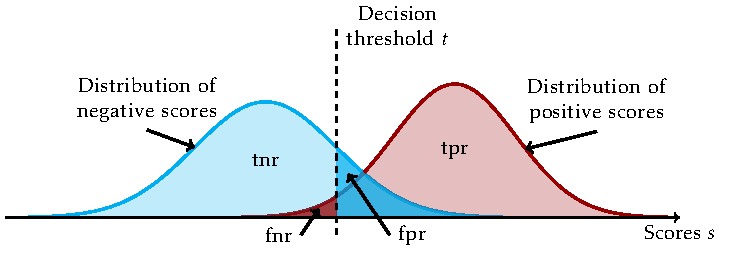
\includegraphics{images/confusion_rates.pdf}
  \caption{The relation between classification scores and  rates. The blue and red curves represent the theoretical distribution of the scores of negative and positive samples, respectively. The area between the blue line and the x-axis is divided by the decision threshold~$t.$ The left part represents a true-negative rate, while the right represents a false-positive rate. The area between the red line and the x-axis is also divided by~$t.$ The left part represents a false-negative rate, and a right represents the true-positive rate.}
  \label{fig: scores and rates}
\end{figure}

The confusion matrix is not the only way to measure the performance of binary classifiers. For example, there are many different classification matrices, and many of them are derived directly from the confusion matrix~\cite{fawcett2006introduction, metz1978basic, brodersen2010balanced, hossin2015review}. As an example, we can mention accuracy and balanced accuracy defined by
\begin{align*}
  \accuracy & = \frac{1}{n}\Brac{\tp + \tn} &
  \baccuracy & = \frac{1}{2}\Brac{\tpr + \tnr}
\end{align*}
Note that the objective function in~\eqref{eq: Binary classification counts} is accuracy if~$\lambda_1 = \lambda_2 = \frac{1}{\nall}.$ Moreover, for~$\lambda_1 = \frac{1}{2\nneg}$ and~$\lambda_2 = \frac{1}{2\npos},$ the objective function is balanced accuracy. This show the importance of these two performance matrices for standard binary classification. More performance metrics derived from the confusion matrix can be found in Table~\ref{tab: classification metrics}. Moreover, in the following section, we introduce a different approach for the performance evaluation of binary classifiers.

\begin{table}
  \centering
  \begin{NiceTabular}{ccc}
    \CodeBefore
      \rowcolor{\headercol}{1}
      \rowcolors{3}{\rowcol}{}[restart]
    \Body
    \toprule
    \textbf{Name} & \textbf{Aliases} & \textbf{Formula} \\
    \midrule
    true negatives
      & correct rejection
      & $\tn$ \\
    false positives
      & Type I error, false alarm
      & $\fp = \nneg - \tn$ \\
    true positives
      & hit
      & $\tp$ \\
    false negatives
      & Type II error
      & $\fn = \npos - \tp$ \\
    \midrule
    true negative rate
      & specificity, selectivity
      & $\tnr = \frac{\tn}{\nneg}$ \\
    false positive rate
      & fall-out
      & $\fpr = \frac{\fp}{\nneg} = 1 - \tnr$ \\
    true positive rate
      & sensitivity, recall, hit rate
      & $\tpr = \frac{\tp}{\npos}$ \\
    false negative rate
      & miss rate
      & $\fnr = \frac{\fn}{\npos} = 1 - \tpr$ \\
    \midrule
    accuracy
      & ---
      & $\accuracy = \frac{\tp + \tn}{n}$ \\
    balanced accuracy
      & ---
      & $\baccuracy = \frac{\tpr + \tnr}{2}$ \\
    precision
      & positive predictive value
      & $\precision = \frac{\tp}{\tp + \fp}$ \\
    \bottomrule
  \end{NiceTabular}
  \caption{Summary of classification metrics derived from confusion matrix. The first column shows the name used in this work, while the second column shows alternative names that can be found in the literature. The last column shows the formula based on the confusion matrix.}
  \label{tab: classification metrics}
\end{table}

\begin{figure}
  \centering
  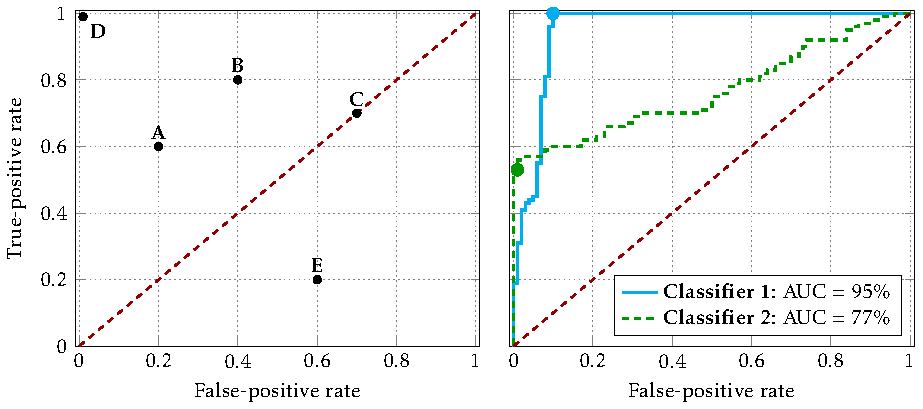
\includegraphics{images/roc_space.pdf}
  \caption{A basic representation of the ROC space with five different classifiers. (\textbf{left}) A comparison of ROC curves for two different classifiers. (\textbf{right})}
  \label{fig: roc space}
\end{figure}

\subsection{ROC Analysis}\label{subsec: ROC}

In the previous section, we defined a general binary classification formulation~\eqref{eq: Binary classification counts} that minimizes a weighted sum of false-positive and false-negative counts. Therefore, we always have to find some trade-off between the false-positive and false-negative counts and select the best hyperparameters~$\lambda_1,$ $\lambda_2,$ for given tasks. There is no universal truth which of these two errors is worse. For example, it is probably better to classify a healthy patient as sick and do additional tests than the other way around. On the other hand, in computer security, an antivirus program with a lot of false-positive alerts is useless since it is disruptive to the user. One way to visualize the trade-off between false-positive and false-negative errors is Receiver Operating Characteristic (ROC) space~\cite{egan1975signal, fawcett2006introduction}.

ROC space is a two-dimensional space with the x-axis equal to the false-positive rate and the y-axis to the true-positive rate. The left-hand side of Figure~\ref{fig: roc space} shows the ROC space with five highlighted points. Each point in the ROC space represents one fixed classifier, i.e., one pair of model~$f$ and decision threshold~$t.$ There are several important points in the ROC space. The point~$(0, 0)$ represents a classifier classifying all samples as negative, while~$(1, 1)$ is a classifier classifying all samples as positive. Both these classifiers are useless. On the other hand, the point (0, 1) represents the perfect classifier that classifies all samples correctly since~$\fpr = 0$ and~$\tpr = 1.$

ROC representation allows us to decide whether one classifier is better than another, only in some cases. For example, in Figure~\ref{fig: roc space}, classifier \textbf{B} is better than classifier \textbf{C} since \textbf{B} has a higher true-positive rate and at the same time a lower false-positive rate. On the other hand, it is impossible to say which classifier is better if one has a higher true-positive rate and the other has a lower false-positive rate. We can see this situation for classifier \textbf{B} and \textbf{A}. In such a case, the preference depends on the given problem, as discussed at the beginning of this section.

Another important part of the ROC space is the diagonal line highlighted in red in Figure~\ref{fig: roc space}. Any classifier that appears on this diagonal provides the same performance as a random classifier. For example, classifier \textbf{C} is represented in ROC space by point~$(0.7, 0.7).$ Such classifier randomly classifies 70\% of samples as positive. Therefore, any classifier that appears in ROC space in the lower right triangle is worse than a random classifier. There are usually no classifiers in this area since any classifier from the lower right triangle can be easily improved. If we negate the decision of such a classifier for every sample, we get its negated version in the upper left triangle. Such a situation is in Figure~\ref{fig: roc space} for classifier \textbf{E} and \textbf{B}. Since classifier \textbf{E} has a false-negative rate of 0.8, we can deduce that negated classifier will have a true-positive rate of 0.8. Similarly, since classifier \textbf{E} has a true-negative rate of 0.4, its negated version will have a false-positive rate of 0.4. Therefore the negated version of classifier \textbf{E} is represented in ROC space by point~$(0.4, 0.8),$ which is classifier~\textbf{B}.

Many classifiers do not provide classification scores and the decision threshold, and instead, perform direct decisions on whether samples are positive or negative. As an example, we can mention decision trees. Such classifiers are always represented as a single point in the ROC space. In this text, we assume that the classifier consists of the model~$f$ that produces classification scores and the decision threshold~$t,$ see Notation~\ref{not: classifier}. Many standard classifiers such as neural networks or logistic regression fall into this setting. Even though the decision threshold is determined during the training process, it is possible to change it and obtain different predictions. This possibility is very often used to produce so-called ROC curves~\cite{fawcett2006introduction}.

ROC curve shows how model~$f$ behaves for different thresholds~$t$ varying from~$-\infty$ to~$+\infty.$ Right-hand side of Figure~\ref{fig: roc space} provides an example of two ROC curves for two different classifiers. \textbf{Classifier 1} provides accuracy~95\% and is represented by the blue dot, while the blue line represents its ROC curve. \textbf{Classifier 2} represented by the green dot provides accuracy~76\%, and the green dashed line represents its ROC curve. A standard method for comparing two classifiers is to compare the corresponding areas under the ROC curves (AUC)~\cite{bradley1997use, hanley1982meaning}. Such an approach is a simple way to reduce the curve to one number. In the case of standard binary classification, the larger the AUC, the better. In Figure~\ref{fig: roc space} we can see that the blue classifier has AUC 95\% while the green one has only 77\%. Therefore, for most classification problems, the blue classifier is better. Even though we get almost the same values of accuracy and AUC for both classifiers, the accuracy is not equivalent to AUC. The similarity is only a consequence of the used example.

Since both false-positive and true-positive rates are non-increasing functions of threshold~$t,$ we can efficiently compute the ROC curve from sorted classification scores. Moreover, the AUC of a classifier is equivalent to the probability that the classifier will rank a randomly chosen positive sample higher than a randomly chosen negative sample~\cite{fawcett2006introduction}. By comparing the classifiers from the right-hand side of Figure~\ref{fig: roc space}, we can deduce that \textbf{Classifier 1} is generally better at a false-positive rate larger than~$0.01.$ Otherwise, \textbf{Classifier 2} is the better one. Therefore,  there is a specific region of the ROC space where \textbf{Classifier 2} outperforms \textbf{Classifier 1}. In the next section, we discuss multiple different problems which focus on the performance only at low false-positive rates.

\section{Classification at the Top}\label{sec: related problems}

As discussed above, \textbf{Classifier 1} focuses on the overall performance, while the  \textbf{Classifier 2} on the performance on low false-positive rates, see Figure~\ref{fig: roc space}. The latter classifier can be handy for search engines such as Google or DuckDuckGo, where the goal is to have all relevant results on the first few pages. The results on page 50 are usually of no interest to anyone, so it is crucial to move the most relevant results to the few first pages~\cite{cortes2003auc}. Therefore, it is essential to push as many positive samples above some small portion of the worst negative samples (negative samples with the largest classification scores). In this section, we use two different visual representations of the performance of classifiers from the right-hand side of Figure A to show the difference and emphasize the advantages of both of them.

Figure~\ref{fig: standard vs. aatp} shows the difference between the standard classifier (\textbf{Classifier 1}) that maximizes the accuracy and the classifier that focuses only on the classification at the top (\textbf{Classifier 2}). In this particular case, \textbf{Classifier 2} maximizes the number of positive samples that are ranked higher or equal than the worst negative sample. In other words, \textbf{Classifier 2} maximizes true-positive rate at the smallest possible false-positive rate. If we go back to the example with search engines, the goal of \textbf{Classifier 2} is to push as many relevant results before the first irrelevant. Formally, \textbf{Classifier 2} maximizes the following metric
\begin{equation}\label{eq: metric pos at top}
  \postop(\bm{s}) = \frac{1}{\npos} \sum_{i \in \Ipos} \Iverson{s_i \geq \max_{j \in \Ineg}s_j}.
\end{equation}
For both classifiers, Figure~\ref{fig: standard vs. aatp} shows two different decision thresholds. The black threshold is the one for which the classifier was trained, while the green one represents the worst negative sample. For \textbf{Classifier 2} these two thresholds coincide. We can observe that \textbf{Classifier 1} provides a much better separation of positive and negative samples. Only a few samples above the black threshold ruin perfect separation. On the other hand, the separation provided by \textbf{Classifier 2} is much worse since half of the positive samples are mixed with negative ones. Therefore, the accuracy of \textbf{Classifier 1} is~$95\%$ while the accuracy of \textbf{Classifier 2} is only~$76\%.$ However, in terms of metric~\eqref{eq: metric pos at top} the situation is quite different. Since there are few negative outliers, there is only 19\% of positive samples above the worst negative for \textbf{Classifier 1}, but 53\% for \textbf{Classifier 2}.

The same behavior can also be demonstrated using ROC curves. Figure~\ref{fig: roc space log} show ROC curves for both classifier with (rihght) and without (left) logaritmic scaling of x-axis. The blue line represents ROC curve for \textbf{Classifier 1} and the green dashed one for \textbf{Classifier 2}. Moreover, There are two important points for \textbf{Classifier 2}. The blue filled circle corresponds to the black threshold and the blue filled square to the green threshold from Figure~\ref{fig: standard vs. aatp}. Since for \textbf{Classifier 2} both thresholds coincide, there is only one point in Figure~\ref{fig: roc space log} highlighted by a green square. The superiority of \textbf{Classifier 1} in the overall performance is evident from the left-hand side of the figure, since there is only a small region of ROC space, where \textbf{Classifier 2} provides a higher true-positive rate. However, this region is very interesting. The right-hand side of Figure~\ref{fig: roc space log} allows us to concentrate on very low false-positive rates. 
If the false-positive rate is lower than~$7 \cdot 10^{-1},$ then \textbf{Classifier 2} provides better true-positive rate than \textbf{Classifier 1}. Finally, the value of metric~\eqref{eq: metric pos at top} is highlighted using squares for both classifiers and it is clear, that \textbf{Classifier 2} provides higher value of this metric.

\begin{figure}
  \centering
  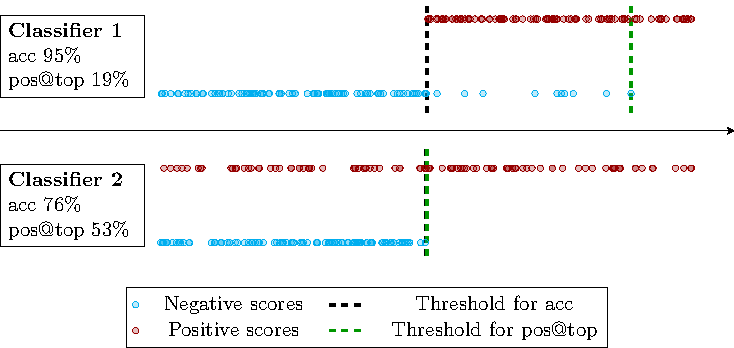
\includegraphics{images/standard_aatp_comparison.pdf}
  \caption{Difference between standard classifiers (\textbf{Classifier~1}) and classifiers maximizing~$\postop$ metric (\textbf{Classifier~2}). While the former has a good total accuracy, the latter has a good~$\postop$ metric.}
  \label{fig: standard vs. aatp}
\end{figure}

\begin{figure}
  \centering
  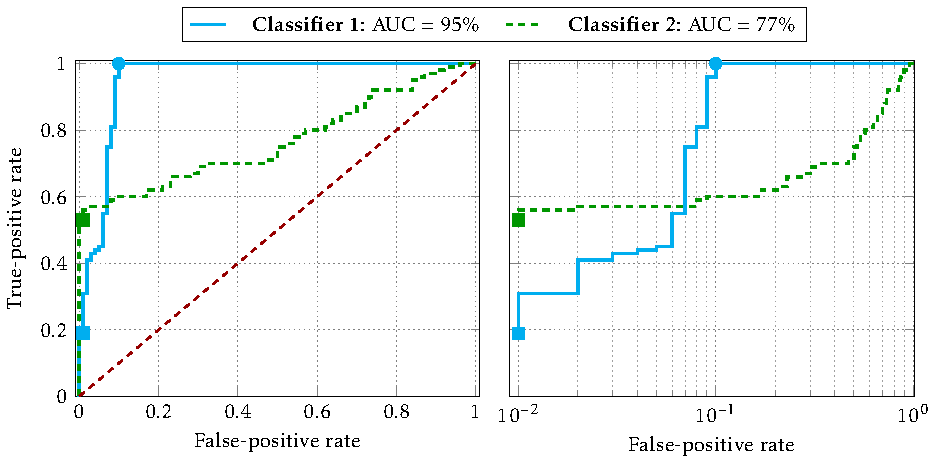
\includegraphics{images/roc_space_log.pdf}
  \caption{Difference between standard classifiers (\textbf{Classifier~1}) and classifiers maximizing~$\postop$ metric (\textbf{Classifier~2}). While the former has a good total accuracy, the latter has a good~$\postop$ metric.}
  \label{fig: roc space log}
\end{figure}

The rest of the chapter presents three main categories of problems that focus only on a small number of the most relevant samples. Moreover, in Chapter~\ref{chap: framework}, we show that at least some formulations from these three categories are closely related to binary classification.

\subsection{Ranking Problems}

The first category is ranking problems. The ranking algorithms play a crucial role in many information retrieval problems:
\begin{itemize}
  \item \textbf{Document (Text) retrieval systems} are used for obtaining relevant documents from the collection of documents based on the relevance to the user's query. Such systems are widely used for accessing books, journals, or any other documents. However, the most visible application is search engines such as Google or DuckDuckGo.
  \item \textbf{Collaborative filtering} is one of the techniques used to predict the user's rating of a new product based on the past ratings of users with similar rating patter. Such systems can be used to generate music or video playlist automatically. Therefore, such systems are widely used in services such as Youtube or Spotify.
\end{itemize}
The two examples above show that ranking problems usually depend on users' feedback or preferences. In binary classification, we have only the labels that represent if the samples are positive or negative. On the other hand, ranking problems use multiple ways to describe the users' feedback. One approach uses the feedback function~$\Phi: \R^d \times \R^d \to \R$ to represent the user's preferences~\cite{freund2003efficient}. In such a case, the feedback function can be defined for all pairs of samples~$(\bm{x}_i, \bm{x}_j)$ in the following way
\begin{equation*}
  \Phi(\bm{x}_i, \bm{x}_j) \; 
  \begin{cases}
    > 0 & \bm{x}_i \text{ is prefered over } \bm{x}_j, \\
    = 0 & \text{no preference,} \\
    < 0 & \bm{x}_j \text{ is prefered over } \bm{x}_i.
  \end{cases}
\end{equation*}
We can see, that the feedback function specify if the user prefers~$\bm{x}_i$ over~$\bm{x}_j$ or not. Moreover, the feedback function also specifies how strong the preference is, i.e., the higher the volume~$\abs{\Phi(\bm{x}_i, \bm{x}_j)},$ the higher the preference. Many ranking algorithms try to find some ordering of all samples that minimizes the number of misordered pairs of samples. Consider ranking function~$r: \R^d \to \R.$ The sample~$\bm{x}_i$ is ranked higher than sample~$\bm{x}_j$ if~$r(\bm{x}_i) > r(\bm{x}_j).$ Then, the minimization of the number of misordered pairs can be formally written as follows
\begin{mini}{r}{
  \sum_{i \in \I} \sum_{j \in \I} \Iverson{r(\bm{x}_i) \leq r(\bm{x}_j)} \cdot \max\Brac[c]{0, \; \Phi(\bm{x}_i, \bm{x}_j)}.
  }{\label{eq: rankboost}}{}
\end{mini}
This problem is hard since the objective function contains a pairwise comparison of all samples. Therefore, the problem is not suitable for large data. \emph{RankBoost}~\cite{freund2003efficient} is an boosting algorithm based on the AdaBoost~\cite{freund1997decision} that combines many weak ordering functions to obtain the final ranking. This approach leads to the maximization of the area under the ROC curve~\cite{rudin2009pnorm}. Therefore, RankBoost focuses on the overall performance. However, as we discussed at the beginning of the section, we want to focus only on the small portion of the most relevant samples in many applications. In such a case, this approach is not ideal.

Consider recommendation of movies. In such a case, we only care about if the movie is good or not. It doesn't matter if one bad movie is ranked higher than another bad movie. Both movies are still bad and therefore not relevant. Many ranking algorithms~\cite{rudin2009pnorm} use the so-called bipartite ranking to address this situation. In such a situation, each sample is positive (good) or negative (bad), and the goal is to push positive samples above negative ones. The authors of~\cite{rudin2009pnorm} proposed the following formulation
\begin{mini}{r}{
  \Brac{\sum_{j \in \Ineg} \Brac{\sum_{i \in \Ipos} \Iverson{r(\bm{x}_i) \leq r(\bm{x}_j)}}^p}^{\frac{1}{p}}.
  }{\label{eq: p-norm push}}{}
\end{mini}
The authors of~\cite{rudin2009pnorm} also proposed boosting algorithm called \textbf{$p$-Norm Push} to solve the formulation above. Note that for~$p = 1$, the formulation~\eqref{eq: p-norm push} is very similar to the RankBoost~\eqref{eq: rankboost}. In such a case, the resulting ranking function maximizes the AUC and therefore optimizing overall rankig. On the other hand, for~$p \rightarrow +\infty$, the formulation~\eqref{eq: p-norm push} minimizes the largest number of positive samples ranked below any negative sample
\begin{mini*}{r}{
  \max_{j \in \Ineg} \; \sum_{i \in \Ipos} \Iverson{r(\bm{x}_i) \leq r(\bm{x}_j)}.
  }{}{}
\end{mini*}
In such a case, the resulting ranking function focus only on the absolute top, i.e., it aims to push as many positive samples above the negative sample with the highest rank. Moreover, the formulation above can be equivalently rewritten as follows
\begin{mini}{r}{
  \sum_{i \in \Ipos} \Iverson{r(\bm{x}_i) \leq \max_{j \in \Ineg} \; r(\bm{x}_j)}.
  }{\label{eq: toppush rank}}{}
\end{mini}
Authors of~\cite{agarwal2011infinite} focus on this formulation and introduces SVM (\emph{Support Vector Machines}~\cite{cortes1995support}) based algorithm called \emph{Infinite Push} to solve it. Finally, authors of~\cite{li2014top} proposed an even more efficient algorithm with the linear complexity in the number of samples called \TopPush. Note that the objective function of the problem above is almost the same as the metric~\eqref{eq: metric pos at top}. Therefore, this \textbf{Classifier 2} from Figures~\ref{fig: standard vs. aatp} and~\ref{fig: roc space log} corresponds to the ranking function given by \TopPush algorithm. It shows a tied connection between binary classification and the bipartite ranking problems. 

\subsection{Accuracy at the Top}

In the previous section, we introduced formulation~\eqref{eq: toppush rank}, which focuses on maximizing the number of positive samples above the worst negative sample (the one with the highest rank or highest classification score). This formulation is very useful, as discussed at the beginning of this section. However, such a maximization problem can be unstable since the objective function does not allow false-positive errors. Therefore, if there is one negative outlier with a high score, the number of positive samples above this outlier can be tiny. The authors of~\cite{boyd2012accuracy} focus on similar problems as \TopPush, but use a different approach. They proposed the following formulation and it called \textbf{Accuracy at the Top}
\begin{mini}{\bm{w}}{
  \frac{1}{\nneg} \fp(\bm{s}, t) + \frac{1}{\npos} \fn(\bm{s}, t)
  }{\label{eq: aatp intro}}{}
  \addConstraint{s_i}{= f(\bm{x}_i; \bm{w}), \quad i \in \I}
  \addConstraint{t}{= \max \Set{t}{\frac{1}{\nall} \sum_{i \in \I} \Iverson{s_i \geq t} \geq \tau},}
\end{mini}
where~$f: \R^d \to \R$ is a model. This formulation focuses on the top $\tau$-fraction of all samples and tries to maximize the number of positive samples and minimize the number of negative samples in it. Even though the goal is to maximize the number of positive samples above the top $\tau$-quantile, the objective function contains false-positive and false-negative rates. It should be sufficient to include only one of them since the definition of the threshold implies the minimization of the other one as well. However, this form of objective function should be more robust~\cite{grill2016learning}. The problem of Accuracy at the Top is useful, for example, in applications where identified samples undergo expensive post-processing, such as human evaluation. For example, potentially useful drugs need to be preselected and manually investigated in drug development. Since the manual investigation is costly, we have to select only a fraction of drugs with the highest potential. However, it is precisely what Accuracy at the Top does.

There are many methods on how to solve Accuracy at the Top, since the formulation is complicated due to the top $\tau$-quantile in the constraint. The early approaches aim at solving approximations. For example, the authors of \cite{joachims2005svm} optimize a convex upper bound on the number of errors among the top samples. Due to exponentially many constraints, the method is computationally expensive. In \cite{boyd2012accuracy} the authors presented an SVM-like formulation. They assume that the top $\tau$-quantile is one of the samples, construct~$n$ unconstrained optimization problems with fixed thresholds, solve them and select the best solution. While this removes the necessity to handle the (difficult) quantile constraint, the algorithm is computationally infeasible for a large number of samples. The authors of~\cite{grill2016learning} proposed the projected gradient descent method, where after each gradient step, the quantile is recomputed. In \cite{eban2017scalable} authors suggested new formulations for various criteria and argued that they keep desired properties such as convexity. Finally, the authors of~\cite{tasche2018plug} showed that Accuracy at the Top is maximized by thresholding the posterior probability of the relevant class.

\subsection{Hypothesis Testing}

The hypothesis testing operates with null~$H_0$ and alternative~$H_1$ hypothesis. The goal is to either reject the null hypothesis in favor of the alternative or not. Since this problem is binary, two possible errors can occur. Type I occurs when~$H_0$ is true but is rejected, and Type II error happens when~$H_0$ is false but fails to be rejected. The Neyman-Pearson problem minimizes~\cite{neyman1933ontheproblem} Type II error while keeping Type I error smaller than some predefined bound. Using our notation for the Neyman-Pearson problem, the null hypothesis~$H_0$ states that sample~$\bm{x}$ has a negative label. Then Type I error occurs when the sample is false-positive, while Type II error occurs when the sample is false-negative. Therefore, the Neyman-Pearson problem minimizes the false-negative rate with the prescribed level~$\tau$ of the false-positive rate. Such constraint can be written in the form of quantile, i.e., the threshold is the top $\tau$-quantile of scores of all negative samples.
\begin{mini*}{f}{
  \frac{1}{\npos} \fn(\bm{s}, t)
  }{}{}
  \addConstraint{s_i}{= f(\bm{x}_i), \quad i \in \I}
  \addConstraint{t}{= \max \Set{t}{\frac{1}{\nneg} \sum_{i \in \Ineg} \Iverson{s_i \geq t} \geq \tau},}
\end{mini*}
This formulation is very similar to the one for Accuracy at the Top~\eqref{eq: aatp intro}. The main difference is that the quantile in the constraint is not computed from all but only from negative samples. Also, note one key difference in interpretation. The~$\tau$ in Accuracy at the Top represents the total amount of samples we want to process with the smallest possible error. On the other hand, in the Neyman-Pearson problem~$\tau$ represents the maximal acceptable false-positive rate. Therefore, the former approach is useful in situations where we can process only a certain number of samples. The latter is for situations where we have strict constraints on false-positive errors.

\section{Summary}

In this chapter, we introduced the general formulation~\eqref{eq: Binary classification counts} for binary classification and discussed how to measure the performance of binary classifiers. The first approach for performance evaluation is based on the confusion matrix. This approach is very straightforward. Moreover, it is possible to derive many different classification matrices from the confusion matrix. Table~\ref{tab: classification metrics} summarizes classification matrices derived from the confusion matrix used in the upcoming chapters. The second approach introduced in this chapter uses the ROC space to visualize the ability of classifiers to rank positive samples above negative ones. Since standard binary classification focuses on optimizing the overall performance, we discussed that there are many problems closely tied to the binary classification that focuses on the performance only of the most relevant samples. Such problems occur in many applications, from search engines to drug development. We also introduced Ranking problems, the problem of Accuracy at the Top, and the Neyman-Pearson problem and discussed their relation to the binary classification. In the upcoming chapters, we focus on these three groups of problems and introduce a general framework to handle them.
